\section{Introduction}
\label{sec:intro}
Optical ghosts are caused by multiple reflections of light off of optical elements with non-zero reflectivity. Although ghosts are created by all astronomical sources, most of them are undetectable and have a negligible impact on astronomical measurements. However, ghosts produced by bright stars can be impactful even if the reflectances of the optical elements are small ($\sim$ 1\%) because the total flux of photons from these stars are large. Figure~\ref{fig:optical_ghosts} shows an example of optical ghosts created by a bright star (CD-62 181) in the top right corner of the LSST Camera focal plane during commissioning of the Vera C.\ Rubin Observatory. 

Ghosts produced by bright stars often pose challenges to sky background estimation and photometric measurements. They are also sources of contamination for low-surface-brightness science \citep[e.g.,][]{Tanoglidis:2021,Tanoglidis:2022}. Measuring the area of the focal plane affected by these artifacts is crucial to assess the impact on these science cases.

The LSST System Requirement\footnote{OSS Requirements: \url{https://docushare.lsst.org/docushare/dsweb/Get/LSE-30};  LSR Requirements: \url{https://docushare.lsst.org/docushare/dsweb/Get/LSE-29} } on the impact of optical ghosts states that the: ``Percentage of image area that can have ghosts with surface brightness gradient amplitude of more than 1/3 of the sky noise over 1 arcsec shall be less than 1\%''. 
The wording of this requirement leaves some room for interpretation. We opt to define the requirement somewhat conservatively as the total area of the focal plane containing a ghost with a flux that is greater than 1/3 of the sky noise on any detector. In order to satisfy this requirement, the total affected area should not exceed 1\%. We also assume that this requirement is intended to apply to the ensemble of visits rather than each individual visit.

Measuring the fluxes of the ghosts with on-sky data to estimate the ghost-flux-to-sky-noise ratio is challenging. Uneven flat-fielding during commissioning led to gradients in the mean sky counts across the focal plane, affecting the sky noise and ghost flux across the ghost. Most of the prominent ghosts were also found to be spatially degenerate, with some ghosts fully overlapping others. This made fitting the amplitude of each individual ghost difficult. To circumvent these challenges, we chose instead to calculate the expected impact of ghosts by performing ray-tracing simulations of known bright stars, taking into account their positions relative to the boresight and approximate brightnesses, as well as the locations of Rubin commissioning observations. The simulated fluxes of the ghosts were compared and calibrated to the Rubin commissioning data to validate this approach.

We use the Collimated Beam Projector \citep[CBP;][]{2016SPIE.9906E..0OI} -- a 30\,cm Schmidt telescope refitted with a laser -- to produce ghosts on the focal plane.
We measure the fluxes of these ghosts and derive estimates for the reflectances of the optical elements (Filter, Detector \& Lenses) of LSSTCam.
These measurements serve as validation of the reflectances used in the simulations where we estimate the area of sky impacted by optical ghosts.

This technote is structured as follows. 
Section~\ref{sec:ghost_impact} delineates the procedure and results of our estimation of the sky area impacted by ghosts.
Section~\ref{sec:reflectances} shows our measurements of the optical reflectances of the telescope optics using ghosts.

\begin{figure}[t!]
    \centering
    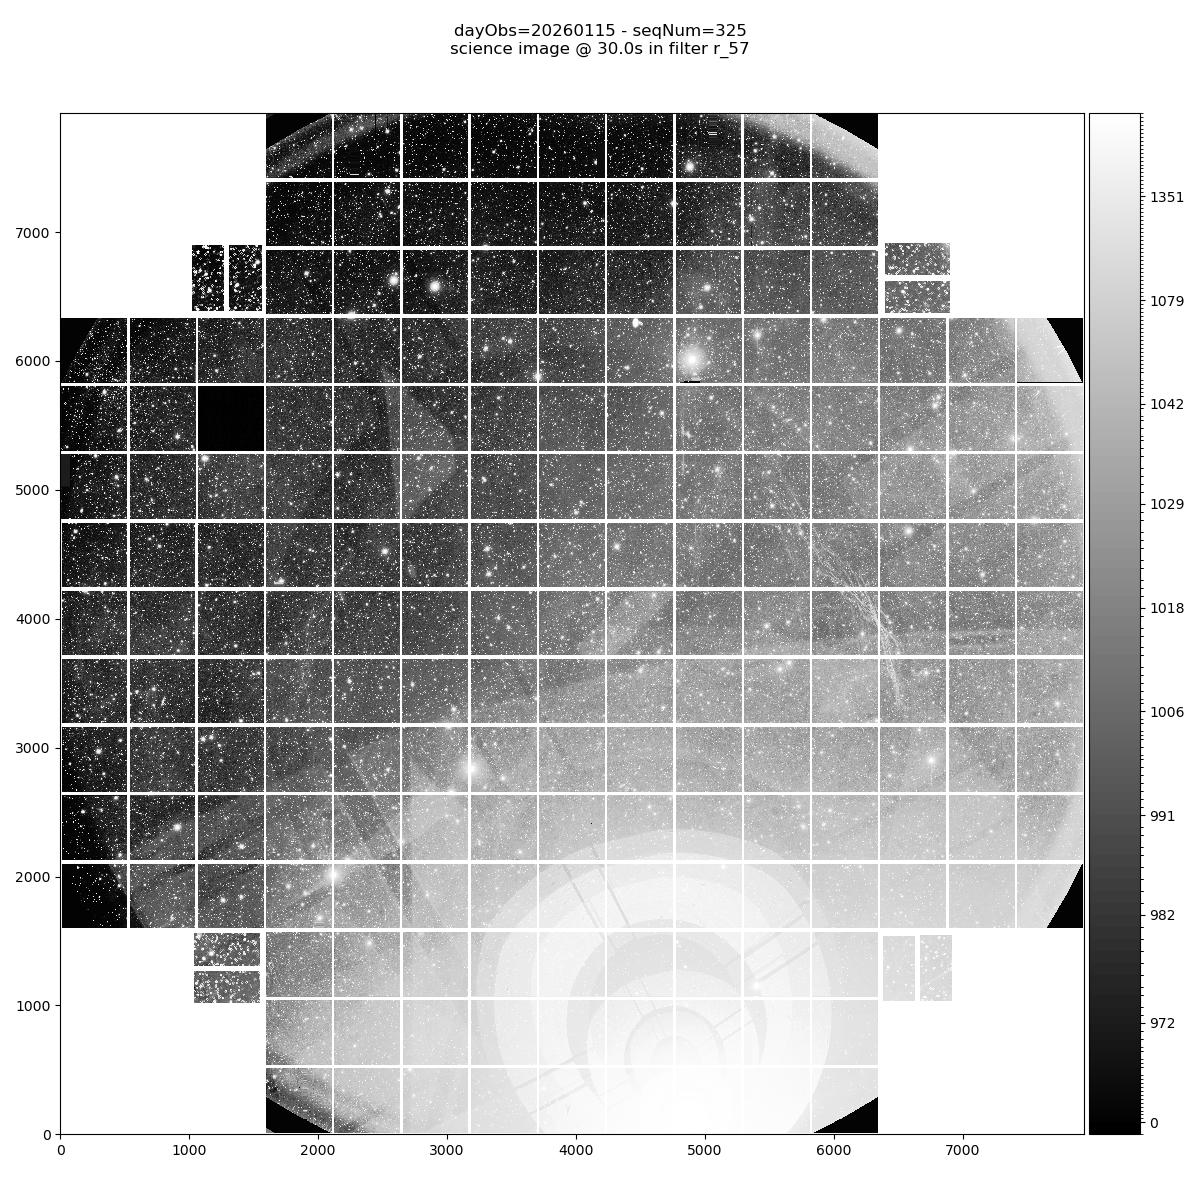
\includegraphics[width=0.4\textwidth]{figures/lsstcam_focal_plane_mosaic_2026-01-15_000325.jpg}
    \caption{Post-ISR image of the LSSTCam focal plane (visit 2026011500325; {\it r} band) with optical ghosts created by a bright star (Canopus/ Alpha Carinae) in the top right corner. } 
    \label{fig:optical_ghosts}
\end{figure}